\chapter{Обзор предметной области и постановка задачи}

\section{Динамическая и статическая трансляция}

\textit{2 страницы}

\begin{Def}\label{binary_translation}
Бинарная трансляция - эмуляция одного набора инструкций через другой набор инструкций, т. е. трансляция последовательности инструкций исходного набора в эквивалентную последовательность инструкций целевого набора комманд.
\end{Def}

В зависимости от необходимости исполнения исходной последовательности иснтрукций бинарную трансляцию разделяют на статическую и динамическую.

Статическая трансляция не подразумевает интерпретацию исходной последовательности, в то время как динамическая трансляция подразумевает интрепретацию исходной последовательности комманд.

Технологии бинарной трансляции используются очень широко, например, вирутальные машины Java и .NET преобразуют байт-код в машинный код целевой платформы, что является частным случаем бинарной трансляции.

QEMU осуществляет бинарную трансляцию для эмуляции набора комманд одного процессора на другом, что позволяет использовать его, например, вместо реального аппартного обеспечения при разработке программных продуктов.

Популярный профилировщик Valgrind осуществляет бинарную трансляции в свое внутренне представление VEX IR~\footnote{http://www.valgrind.org/docs/manual/writing-tools.html}, в котором проще инструментировать код.

\subsection{Статическая трасляция}

В связи с необходимости сохранения семантики исходной последовательности комманд, например, атомарность определенных инструкций, статическая трансляция является довольно сложной, кроме того, как я уже писал выше, имея только исполняемый файл в общем случае нельзя отличить бинарный код от данных программы без интерпретации бинарного кода, что ограничивает применение этого подхода.

Существуют различные реализации статических трансляторов, например, Ngen~\footnote{http://en.wikipedia.org/wiki/Native\_Image\_Generator} производит статическую трансляцию CIL в бинарный код целевой платформы, аналогичные средства есть для байт-кода Java~\footnote{http://en.wikipedia.org/wiki/GNU\_Compiler\_for\_Java}~\footnote{http://en.wikipedia.org/wiki/Excelsior\_JET}.

Следует отметить, что технологии статической трансляции могут применяться не только для преобразования последовательностей инструкций из разных наборов комманд, но и для преобразования последовательности комманд в рамках одного набора инструкций, например, с целью оптимизации~\footnote{http://www.cs.arizona.edu/projects/alto/}.

\subsection{Динамическая трансляция}

По сравнению со статической динамическая трансляция имеет меньше ограничений, но за большую свободу часто приходится платить меньшей производительностью из-за накладных расходов на интерпретацию, которых нет при статической трансляции.

Однако не всегда производительность динамической трансляции ниже. Для ускорения может применяться техника Just In Time (JIT) компиляции, когда последовательности инструкций исходной платформы компилируются "на лету" в набор инструкций целевой платформы, что уменьшает накладные расходы. Кроме того при использовании JIT возможно использование оптимизаций недоступных при статической трансляции. Так JIT компилятору доступна, например, информация о наиболее горячих участках программы, что позволяет сгенерировать более оптимальный, по сравнению со статически сгенерированным, бинарный код.

В качестве примеров динамических трансляторов можно привести вирутальные машины Java и .NET, а в качестве примера транслятора нативного кода QEMU и Valgrind.

В своей работе в качестве динамическго транслятора я использую QEMU, так как он поддерживает множество аппаратных платформ (в том числе и arm), а кроме того имеет режим User Mode (для Linux и Free BSD), в котором он виртуализует не целую вычислительную систему, а только окружение одного процесса и осуществляет трансляцию системных вызовов исходной платформы (в рамках моей работы x86) в системные вызовы целевой (в рамках моей работы arm).

\section{Существующие реализации миграции}

Как я уже писал выше, существуют различные реализации технологий миграции процессов, далее коротко будут рассмотрены 4 наиболее близких к моей работе.

\subsection{Linux-cr}
\label{linux_cr}

Проект по реализации технологии checkpoint/restore в ядре Linux~\footnote{https://ckpt.wiki.kernel.org/index.php/Main\_Page}. На данный момент проект не выглядит активным, последняя активность в ноябре 2010 года~\cite{linux_cr_lwn_report}. На момент последней актвности код состоял из около 100 патчей в ядро Linux и содержал порядка 23 000 строк кода.

Основной проблемой проекта была попытка реализации проекта в пространстве ядра, так как он затрагивает большое количество подсистем, что усложняет поддержку и развитие проекта, а ошибки в системе миграции влияют на работу всей системы, делая ядро хрупким. Именно поэтому в своей работе я стараюсь минимизировать вмешательство в ядро Linux и получить как можно больше информации в пространстве пользователя.

Проект обладает достаточно большим списком поддерживаемых фич, кроме того поддерживает несколько архитектур: x86, x86\_64, PowerPC, s390 и arm.

Список поддерживаемых фич:

\begin{itemize}

    \item поддержка многопоточных программ
    \item поддержка фьютексов
    \item поддержка сигналов
    \item файловые дескрипторы и директории для различных файловых систем
    \item файлы устройств (/dev/null, /dev/zero, /dev/random, /dev/urandom)
    \item поддержка epoll и event
    \item поддержка сокетов unix, ipv4 и ipv6 сокетов

\end{itemize}

но даже этот спсиок не описывает все ресурсы, которые необходимо поддержать для полноценной миграции процессов.

\subsection{CRIU}

CRIU проект по реализации технологии checkpoint/restore преимущественно в пространстве пользователя Linux~\footnote{http://criu.org/Main\_Page}. Проект развивается при поддержке компании Paralles и находится в активной разработке.

Поддерживаемые фичи:

\begin{itemize}

    \item сохранение и восстановление TCP соединений
    \item сохранение и восстановление файловых дескрипторов
    \item поддрежка многопоточных программ
    \item поддержка со стороны mainstream ядра

\end{itemize}

К сожалению, CRIU поддердивает только платформу x86\_64, что делает его неприменимым для кросс-архитектурной миграции процессов.

\subsection{DMTCP}

Проект по реализации технологии checkpoint/restart на уровне библиотек~\footnote{http://dmtcp.sourceforge.net/index.html}. Проект развиватеся, возможно, не очень активно, последняя версия 1.2.7 выпущена 13 марта 2013 года. Принцип работы заключается в запуске целевого процесса в специальном окружении, которое позволяет перехватывать некоторые вызовы и таким образом отслеживать состояние. DMTCP реализован в пространстве пользователя и поддерживает как многопоточные так и распределенные системы.

В связи с тем, что отслеживание состояния происходит во время работы процесса за счет перехвата библиотечных вызовов, существует некоторо падение производительности. Кроме того возможности этого проекта нужно оценивать уже не на уровне ресурсов ОС, а на уровне поддерживаемых библиотек и приложений.

На данный момент, DMTCP поддерживает следующие приложения и библиотеки:

\begin{itemize}

    \item OpenMPI (в частности MPICH2)
    \item MATLAB
    \item Python
    \item Perl
    \item GNU screen
    \item X Window приложения без расширений (например, без OpenGL)
    \item и многие другие

\end{itemize}

Следует отметить, что такая реализация потенциально небезопасна~\footnote{http://criu.org/Comparison\_to\_other\_CR\_projects}. Например, DMTCP умеет перехватывать библиотечный вызов getpid, возвращая ненастоящий pid процесса, но если, этот идентификатор используется для доступа, например, к файловой системе proc. В этом случае, без дополнительной трансляции имен файлов, процесс попытается обратиться к неправильному файлу - файлу другого процесса или несуществующему файлу, хотя в случае поддержки на уровне приложений, это, вероятно, не является проблемой.

\subsection{BLCR}

Проект по реализации checkpoint/restart лаборатории Berkeley~\footnote{https://ftg.lbl.gov/projects/CheckpointRestart/}. Проект направлен на гибридную (пространство пользователя/пространство ядра) реализацию checkpoint/restart не требующую изменения в коде приложения. Проект сосредоточен на параллельных и распределенных приложениях использующих MPI. Поддержка в ядре Linux не требует внесения специальных изменений в ядро и поставляется в вижде набора модулей ядра.

Проект не выглядит активным, последняя версия 0.8.4 вышла 11 октября 2011 года, и начиная с 2008 года изменения содержат только исправления ошибок.

На момент последней активности проект имел стабильную поддержку архитектур x86 и x86\_64, а также эксперементальную поддержку PowerPC, PowerPC64 и arm, но кросс-архитектурная трансляции не поддерживается. Кроме того, как и DMTCP проект требует предварительно загрузки вспомогательных библиотек вместе с целевым процессом.

\section{Цель работы}

\textit{1 страница}

Целью моей работы является реализация технологии кросс-архитектурной трансляции процессов ОС Linux с архитектуры x86 на arm на основе динамического транлятора QEMU. Для достижения указанной цели необходимо решить следующие задачи:

\textbf{\textit{Анализ существующих решений.}} Необходимо рассмотреть существующие реализации технологии миграции процессов, а также принципы работы динамического транслятора QEMU.

\textbf{\textit{Реализация технолигии останова процесса и создания образа.}} Необходимо реализовать технологию создания образа процесса, сохраняющую минимально необходимый для восстановления набор ресурсов процесса - память и состояние регистров процессора. Основными принципами, которых нужно придерживаться при проектировании являются:

\begin{itemize}

    \item минимальное вмешательство в ядро Linux. Причиной этому является неудачный опыт проекта Linux-cr (см.~\ref{linux_cr}), в котором изменения затрагивали очень большое количество подсистема ядра, что сделало проект трудно поддерживаемым.

    \item минимальная поддержка со стороны процесса. Конечная цель разработки технологии миграции перенос как можно большего количества процессов, поэтому минимизация поддержки со стороны самого процесса разумное требование.

    \item архитектура расширяемая на новые платформы. В ходе работы рассматривается только миграция с архитектуры x86 на arm, так как у меня в наличии arm устройство, на котором можно тестировать результаты работы, однако технология кросс-архитектурной миграции не должна ограничиваться только двумя платформами.

\end{itemize}

\textbf{\textit{Реализация восстановления процесса по образу.}} Необходимо реализовать восстановление процесса в динамическом трансляторе QEMU портированном на архитектуру arm.

\textbf{\textit{Тестирование производительности.}} Динамическая трансляция, несомненно, создает overhead, кроме того, процессоры архитектуры arm, как правило, менее производительны, чем процессоры x86, а численные оценки потерь производительности могут дать представление о границах применимости разрабатываемой технологии.

\section{Ресурсы процесса}

\begin{Def}\label{process}
Процесс - контейнер ресурсов операционной системы.
\end{Def}

Согласно определению~\ref{process}, миграция процесса - перенос ресурсов между вычислительными системами, вот далеко не полный перечень ресурсов, которые необходимо переносить:

\begin{itemize}

    \item память
    \item контекст процесса
    \item открытые файлы и директории (обычные и файлы устройств)
    \item сокеты
    \item мьютексы
    \item различные IPC примитивы

\end{itemize}

Для переноса самого простого процесса я сосредоточился только на двух ресурсах: память и состояние процессора. Эти два ресурса обязательно есть у любого процесса в системе, без них работа процесса невозможна. Далее я подробнее рассмотрю некоторые из перечисленных ресурсов процесса. 

\subsection{Память процесса Linux}

\begin{figure}[h]
\center{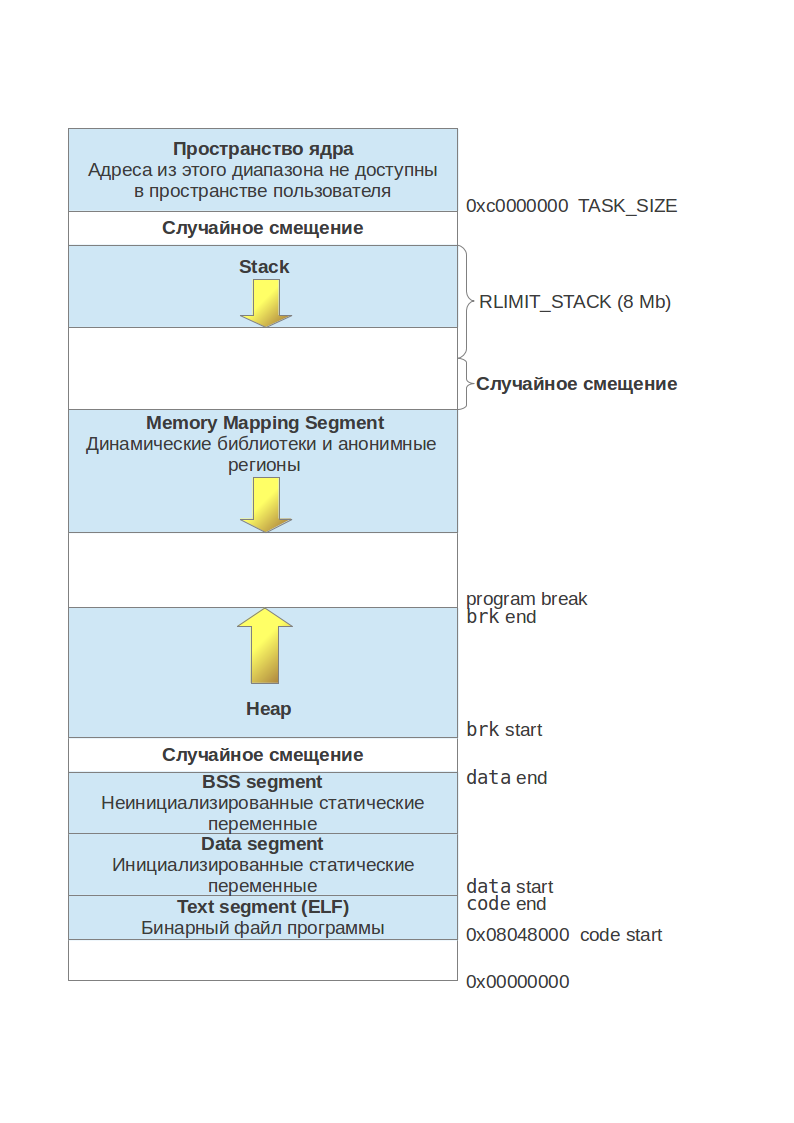
\includegraphics[width=0.6\linewidth]{memory_layout}}
\caption{Типичное размещение регионов памяти процесса ОС Linux на 32 разрядной архитектуре x86}
\label{pic:memory_layout}
\end{figure}

В ОС Linux процессы используют плоскую модель памяти, т. е. любая ячейка памяти адресуется числом (например, в диапазоне от 0x08048000 до 0xc0000000), однако эта память используется неравномерно, типичное использование памяти представлено на рис.~\ref{pic:memory_layout}.

Структура памяти определяется ядром Linux и задается во время создания процесса. Каждому процессу в ядре соответсвует структура task\_struct, которая содержит указатель на структуру mm\_struct - дескриптор памяти процесса.

\begin{lstlisting}[caption=Выборка из структуры struct mm\_struct, label=code:mm_struct]
struct mm_struct {
    struct vm_area_struct * mmap;           /* list of VMAs */

    ...

    struct vm_area_struct * mmap;           /* list of VMAs */
    struct rb_root mm_rb;
    struct vm_area_struct * mmap_cache;     /* last find_vma result */

    ...

    unsigned long mmap_base;                /* base of mmap area */
    unsigned long task_size;                /* size of task vm space */

    ...

    unsigned long start_code, end_code, start_data, end_data;
    unsigned long start_brk, brk, start_stack;

    ...
};
\end{lstlisting}

Основные поля описывающие структуру памяти процесса (см. листинг~\ref{code:mm_struct} и рис.~\ref{pic:memory_layout}):

\begin{itemize}

    \item mmap - указатель на голову списка дескрипторов регионов памяти процесса
    \item mmap\_base - указывает на начало Memory Mapping Segment.
    \item start\_code и end\_code описывают регион, в который был загружен код программы
    \item start\_data и end\_data описывают регион, в который были загружены данные
    \item start\_brk и brk описывают кучу процесса
    \item start\_stack указывает на начало сегмента стека программы

\end{itemize}

\subsection{Контекст процесса}

Контекст процесса описывает состояние процесса, в контекст входит следующая информация:

\begin{itemize}

    \item состояние регистров общего назначения
    \item состояние сопроцессоров и расширений (например, FPU, MMX/SSE)
    \item состояние сегментных регистров
    \item состояние управляющих регистров (например, cr3 или eflags)
    \item указатели стека и комманд

\end{itemize}

В данной работе сохраняется минимальный набор информации, необходимый для восстановления процесса, который включает в себя регистры общего назначения (ebx, ecx, edx, esi, edi, ebp, eax), указатели стека и комманд (esp и eip), а также регистр флагов (eflags).

\subsection{Файлы}

\textit{0.5 страницы}

Файл, с точки зрения пользовательского приложения, просто неотрицательное число - файловый дескриптор и набор функций для манипулирования (open, close, read, write, ioctl и др.). Однако внутри операционной системы файлу может соответствовать как реальный файл хранящийся на диске так и виртуальный файл устройства, единый интерфейс является частью идеологии Unix - "все есть файл", однако состояния обычных файлов и файлов устройств описываюся различными структурами и сохранятся должны по разному. Более того сохранение состояния файла устройства в общем виде вообще невозможно.

Стоит отметить, что файловый дескриптор может идентифицировать не только файлы, но и директории, сокеты, пайпы, общую память и различные другие ресурсы системы, состояние каждого из которых внутри ядра операционной системы описывается своей структурой, но для пользователя для работы с ними предоставляется похожие интерфейсы.


\subsection{Сокеты}

\textit{0.5 страницы}

Сокеты еще один важный ресурс процесса операционной системы Linux. Сохранение и восстановление состояния сокетов - это отдельная большая задача.

Сокеты, как правило, используются как интерфейс для организации сетевого взаимодействия, т. е. они затрагивают не только мигрируемый процесс, но и удаленный процесс, который ничего не знает о миграции. Кроме того, за интерфейсом сокетов скрывается сетевая подсистема Linux, которая поддерживает огромное количество разнообразных протоколов (каждый из которых может иметь свое состояние) и затрагивает большое количество других подсистем ядра.

Стоит также отметить, что интерфейс сокетов используется не только для организации сетевого взаимодействия, например, NETLINK сокеты используются для организации взаимодействия пользовательского процесса и ядра Linux (например, через NETLINK сокеты расылается информация о подключенных к компьютеру usb устройствах).
